%%%%%%%%%%%%%%%%%%%%%%%%%%%%%%%%%%%%%%%%%
% Masters/Doctoral Thesis 
% LaTeX Template
% Version 2.5 (27/8/17)
%
% This template was downloaded from:
% http://www.LaTeXTemplates.com
%
% Version 2.x major modifications by:
% Vel (vel@latextemplates.com)
%
% This template is based on a template by:
% Steve Gunn (http://users.ecs.soton.ac.uk/srg/softwaretools/document/templates/)
% Sunil Patel (http://www.sunilpatel.co.uk/thesis-template/)
%
% Template license:
% CC BY-NC-SA 3.0 (http://creativecommons.org/licenses/by-nc-sa/3.0/)
%
%%%%%%%%%%%%%%%%%%%%%%%%%%%%%%%%%%%%%%%%%

%----------------------------------------------------------------------------------------
%	PACKAGES AND OTHER DOCUMENT CONFIGURATIONS
%----------------------------------------------------------------------------------------

\documentclass[
12pt, % The default document font size, options: 10pt, 11pt, 12pt
%oneside, % Two side (alternating margins) for binding by default, uncomment to switch to one side
english, % ngerman for German
singlespacing, % Single line spacing, alternatives: onehalfspacing or doublespacing
%draft, % Uncomment to enable draft mode (no pictures, no links, overfull hboxes indicated)
%nolistspacing, % If the document is onehalfspacing or doublespacing, uncomment this to set spacing in lists to single
%liststotoc, % Uncomment to add the list of figures/tables/etc to the table of contents
%toctotoc, % Uncomment to add the main table of contents to the table of contents
%parskip, % Uncomment to add space between paragraphs
%nohyperref, % Uncomment to not load the hyperref package
headsepline, % Uncomment to get a line under the header
%chapterinoneline, % Uncomment to place the chapter title next to the number on one line
%consistentlayout, % Uncomment to change the layout of the declaration, abstract and acknowledgements pages to match the default layout
]{DissertationThesis} % The class file specifying the document structure

\usepackage[utf8]{inputenc} % Required for inputting international characters
\usepackage[T1]{fontenc} % Output font encoding for international characters

\usepackage{mathpazo} % Use the Palatino font by default
\usepackage[nodayofweek]{datetime}

\usepackage[backend=bibtex,style=numeric,citestyle=numeric,natbib=true]{biblatex} % Use the bibtex backend with the authoryear citation style (which resembles APA)

%\usepackage[none]{hyphenat}

\addbibresource{bibliography.bib} % The filename of the bibliography

\usepackage[autostyle=true]{csquotes} % Required to generate language-dependent quotes in the bibliography

\usepackage{listings}

%----------------------------------------------------------------------------------------
%	MARGIN SETTINGS
%----------------------------------------------------------------------------------------

\geometry{
	paper=a4paper, % Change to letterpaper for US letter
	inner=2.5cm, % Inner margin
	outer=3.8cm, % Outer margin
	bindingoffset=.5cm, % Binding offset
	top=1.5cm, % Top margin
	bottom=1.5cm, % Bottom margin
	%showframe, % Uncomment to show how the type block is set on the page
}

%----------------------------------------------------------------------------------------
%	THESIS INFORMATION
%----------------------------------------------------------------------------------------

\thesistitle{LAN Level Parental Control} % Your thesis title, this is used in the title and abstract, print it elsewhere with \ttitle
\supervisor{Dr. Dan Cojocar} % Your supervisor's name, this is used in the title page, print it elsewhere with \supname
\examiner{} % Your examiner's name, this is not currently used anywhere in the template, print it elsewhere with \examname
\degree{Master's degree} % Your degree name, this is used in the title page and abstract, print it elsewhere with \degreename
\author{Sergiu Breban} % Your name, this is used in the title page and abstract, print it elsewhere with \authorname
\addresses{} % Your address, this is not currently used anywhere in the template, print it elsewhere with \addressname

\subject{Biological Sciences} % Your subject area, this is not currently used anywhere in the template, print it elsewhere with \subjectname
\keywords{} % Keywords for your thesis, this is not currently used anywhere in the template, print it elsewhere with \keywordnames
\university{\href{http://www.ubbcluj.ro/ro/}{BABEŞ-BOLYAI UNIVERSITY CLUJ-NAPOCA}} % Your university's name and URL, this is used in the title page and abstract, print it elsewhere with \univname
\department{SPECIALIZATION DISTRIBUTED SYSTEMS IN INTERNET} % Your department's name and URL, this is used in the title page and abstract, print it elsewhere with \deptname
\group{\href{}{SPECIALIZATION DISTRIBUTED SYSTEMS IN INTERNET}} % Your research group's name and URL, this is used in the title page, print it elsewhere with \groupname
\faculty{\href{http://www.cs.ubbcluj.ro/}{FACULTY OF MATHEMATICS AND COMPUTER SCIENCE}} % Your faculty's name and URL, this is used in the title page and abstract, print it elsewhere with \facname

\AtBeginDocument{
\hypersetup{pdftitle=\ttitle} % Set the PDF's title to your title
\hypersetup{pdfauthor=\authorname} % Set the PDF's author to your name
\hypersetup{pdfkeywords=\keywordnames} % Set the PDF's keywords to your keywords
}

\newdateformat{monthyear}{\monthname[\THEMONTH] \THEYEAR}

\begin{document}

\frontmatter % Use roman page numbering style (i, ii, iii, iv...) for the pre-content pages

\pagestyle{plain} % Default to the plain heading style until the thesis style is called for the body content

%----------------------------------------------------------------------------------------
%	TITLE PAGE ENGLISH
%----------------------------------------------------------------------------------------

\begin{titlepage}
\begin{center}

\vspace*{.06\textheight}
{\scshape\LARGE \univname\par}\vspace{1.5cm} % University name

\facname\\\deptname\\[2cm] % Research group name and department name

\textsc{\Large DISSERTATION THESIS}\\[0.5cm] % Thesis type

\HRule \\[0.4cm] % Horizontal line
{\huge \bfseries \ttitle\par}\vspace{0.4cm} % Thesis title
\HRule \\[1.5cm] % Horizontal line
 
\begin{minipage}[t]{0.4\textwidth}
\begin{flushleft} \large
\emph{Author:}\\
\authorname % Author name - remove the \href bracket to remove the link
\end{flushleft}
\end{minipage}
\begin{minipage}[t]{0.4\textwidth}
\begin{flushright} \large
\emph{Supervisor:} \\
\href{http://www.cs.ubbcluj.ro/~dan/}{\supname} % Supervisor name - remove the \href bracket to remove the link  
\end{flushright}
\end{minipage}\\[3cm]
 
\vfill

{\large \monthyear\today}\\[4cm] % Date
%\includegraphics{Logo} % University/department logo - uncomment to place it
 
\vfill
\end{center}
\end{titlepage}

%----------------------------------------------------------------------------------------
%	TITLE PAGE ROMANIAN
%----------------------------------------------------------------------------------------

\begin{titlepage}
\begin{center}

\vspace*{.06\textheight}
{\scshape\LARGE{\href{http://www.ubbcluj.ro/ro/}{UNIVERSITATEA BABEŞ-BOLYAI CLUJ-NAPOCA}}\par}\vspace{1.5cm} % University name

{\href{http://www.cs.ubbcluj.ro/}{FACULTATEA DE MATEMATICǍ ŞI INFORMATICǍ}}\\{SPECIALIZAREA SISTEME DISTRIBUITE ÎN INTERNET}\\[2cm] % Research group name and department name

\textsc{\Large LUCRARE DE DISERTAŢIE}\\[0.5cm] % Thesis type

\HRule \\[0.4cm] % Horizontal line
{\huge \bfseries {Control parental la nivelul rețelei locale}\par}\vspace{0.4cm} % Thesis title
\HRule \\[1.5cm] % Horizontal line
 
\begin{minipage}[t]{0.4\textwidth}
\begin{flushleft} \large
\emph{Absolvent:}\\
Breban Sergiu % Author name - remove the \href bracket to remove the link
\end{flushleft}
\end{minipage}
\begin{minipage}[t]{0.4\textwidth}
\begin{flushright} \large
\emph{Conducător ştiinţific:} \\
\href{http://www.cs.ubbcluj.ro/~dan/}{Dr. Cojocar Dan} % Supervisor name - remove the \href bracket to remove the link  
\end{flushright}
\end{minipage}\\[3cm]
 
\vfill

{\large {Iunie 2018}}\\[4cm] % Date
%\includegraphics{Logo} % University/department logo - uncomment to place it
 
\vfill
\end{center}
\end{titlepage}

%----------------------------------------------------------------------------------------
%	ABSTRACT PAGE
%----------------------------------------------------------------------------------------

\begin{abstract}
\addchaptertocentry{\abstractname} % Add the abstract to the table of contents
The Thesis Abstract is written here (and usually kept to just this page). The page is kept centered vertically so can expand into the blank space above the title too\ldots
\end{abstract}

%----------------------------------------------------------------------------------------
%	LIST OF CONTENTS/FIGURES/TABLES PAGES
%----------------------------------------------------------------------------------------

\tableofcontents % Prints the main table of contents

\listoffigures % Prints the list of figures

\listoftables % Prints the list of tables

%----------------------------------------------------------------------------------------
%	THESIS CONTENT - CHAPTERS
%----------------------------------------------------------------------------------------

\mainmatter % Begin numeric (1,2,3...) page numbering

\pagestyle{thesis} % Return the page headers back to the "thesis" style

% Include the chapters of the thesis as separate files from the Chapters folder
% Uncomment the lines as you write the chapters

% Chapter 1

\chapter{Introduction} % Main chapter title

\label{Chapter1} % For referencing the chapter elsewhere, use \ref{Chapter1} 

%----------------------------------------------------------------------------------------

% Define some commands to keep the formatting separated from the content 
\newcommand{\keyword}[1]{\textbf{#1}}
\newcommand{\tabhead}[1]{\textbf{#1}}
\newcommand{\code}[1]{\texttt{#1}}
\newcommand{\file}[1]{\texttt{\bfseries#1}}
\newcommand{\option}[1]{\texttt{\itshape#1}}

%----------------------------------------------------------------------------------------

\section{Parental controls}

\subsection{Overview}
Parental controls developed in the digital era as a means to allow parents to restrict the access of content to their children and may be included in digital television services, computer and video games and mobile devices. The content may not be appropriate for their age and is aimed more at adult audiences. The characteristics of inappropriate content depends for each parent, and is also correlated with the child's age and maturity level and includes information and images that can upset the child, inaccurate information or information that can cause dangerous behavior. Some of this content could be:

\begin{itemize}
\item pornographic material
\item content containing swearing
\item sites that encourage vandalism
\item pictures, videos or games which shows images of violence
\item gambling sites
\item unmoderated chatrooms
\end{itemize}

It is very easy for the child to stumble upon unsuitable sites by accident on any internet enabled device, like mobile phone or tablet and it can be difficult to monitor and filter the content. \parencite{innapropriateContent}

Parental control solutions fall into four categories:

\begin{itemize}
\item content filters, which limit access to different types of inappropriate content
\item usage control, which works by constraining the usage of certain devices by placing time-limits on usage or forbid some types of usage
\item computer usage management tools, which enforces the use of certain software
\item monitoring, which can track the activity when using the devices
\end{itemize}

The rising availability of the Internet increased the demand for methods of parental control that restrict content. Mobile phones offer the most convenient and constant method for content access, and teens ages 13 to 17 are going online frequently. A study by Pew Research Center found that 92\% of teens report going online daily, 24\% of which are using the internet almost constantly, 56\% going online several times a day and 12\% reporting once a day use. Only 6\% go online weekly and 2\% less often. \parencite{lenhart2015teens}

\begin{figure}[th]
\centering
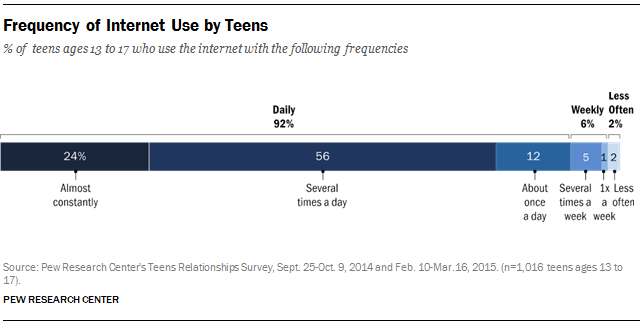
\includegraphics[width=1\textwidth]{Figures/frequency-of-internet-use-by-teens}
\decoRule
\caption[Frequency of Internet Use by Teens]{Frequency of Internet Use by Teens}
\label{fig:frequency-of-internet-use-by-teens}
\end{figure}

The same study finds that nearly three-quarters have or have access to a smartphone and only 30\% have a basic phone and 12\% of teens 13 to 17 have no cell phone of any type.

\subsection{Techniques}

There are two types of control techniques, behavioral control, which consists of controlling the amount of time and how much the child can view, and psychological control, which involves parents tying to influence children by affecting their emotional side by manipulating or insensitivity. Adult control can be divided into three prototypes, each of which has influenced greatly the child-rearing practices \parencite{baumrind1966effects}:

\begin{itemize}
\item permissive: the parent attempts to behave in a nonpunitive, acceptant and affirmative manner and consult with the child about policy decisions and gives explanations for rules
\item authoritarian: the parent attempts to shape, control and evaluate the behavior of the child in accordance with a set standard of conduct, by valuing obedience as a virtue and favoring punitive, forceful measures to curb self-will
\item authoritative: the parent attempts to direct the child's activities in a rational manner, by sharing the reasoning behind the policy and soliciting the child's objections when he refuses to conform; disciplined conformity and autonomous self-will are valued by the authoritative parent
\end{itemize}

Several techniques exists for creating parental controls to block certain websites. Parental control software can monitor API to observe applications such as web browsers or chat applications and to intervene based on certain criteria, such as time based criteria or as a match in a database of banned words. Other techniques that involve a proxy server are also used, in which the proxy server serve as an intermediary which can intervene in the delivery of some content based on various criteria based on the content, but this method has a major disadvantage because it requires client configuration to use the service, which can be easily bypassed.

The difference between content filters and computer usage management methods is that the later is focused on empowering the parents to balance the computing environment for children, by allowing parents to enforce the learning component into the computing time of children, where children can earn play time by working through educational content. This method is very powerful because it stimulates self-regulation in children, instead on relying solely on parental control, and we will use some ideas from this method to develop our control and regulation system.

Recently, some devices which are used for network based parental control have emerged. These devices use different methods to block inappropriate content, such as packet filtering, DNS Response Policy Zone (RPZ) and Deep packet inspection (DPI), and work as a firewall router. Some commercial and governmental communication networks use these methods also, but these type of devices were developed for home also, and are used to create a new home wireless network specifically designed for kids to connect to. We developed our system using the same approach, by creating a custom wireless network for different type of users, different age level children and parents, and by using the packet filtering and DNS techniques to manage content filters.

\subsection{Content filters}

The increased use of mobile devices has created a demand for parental controls for these devices. The first carrier which offered age-appropriate content filters was Verizon, in 2007. With the release of iPhone OS 3.0 in 2009, Apple introduced a mechanism to create age brackets for users, to block unwanted applications from being downloaded. Filtering options are also offered by most internet providers, to limit internet browsing options and block unsuitable content. The software used to restrict or control the content a user is capable to access is commonly referred to as internet filter or content filter.

The content access restrictions can be applied at different levels, from governments applying them nationwide, to ISP blocking it's clients and by a parent to a child's computer. The implementation of this content filtering mechanism can be done at different levels also, by software on the client computer, by using the network infrastructure such as proxy servers, DNS servers or firewall, but none of these solutions alone provides complete coverage, so a mix of technologies have to be used to achieve proper content control.

\begin{itemize}
\item Browser based filters are the most lightweight solution, and the filtering is done by using a third-party browser extension
\item E-mail filters are commonly implemented using a statistical method, Bayesian filters, by acting on information contained in the mail body, headers or attachments
\item Client side filters work by installing it as software on each target device
\item Content-limited (or filtered) ISPs are service providers that offer access to only a set of Internet content, to implement government, regulatory or parental control over its subscribers
\item Network-based filtering is done at the transport layer, by implementing a transparent proxy, redirecting user requests to it by a switch or a router, or at the application layer, by configuring the client to send requests directly to the proxy server. \parencite{contentGateway}
\item DNS-based filtering is implemented at the DNS layer and works by preventing lookups for domains that do not fit within a set of rules, parental control or company rules
\item Search-engine filters work by filtering out inappropriate search results, but if the client knows the URL for a specific content, he can access it without using a search engine; search providers offers child friendly versions of their engines, which filter content inappropriate for children from the search results
\end{itemize}

We implement a DNS-based filtering mechanism, to be able to easily filter out the content that is definitely harmful for a child and does not bring any value, while not being too restrictive and giving the children room to explore and find by themselves what values means and how the time is best spent on the device. The main reason for filtering is to protect the user from harmful content, but it is used also to block malware and other intrusive material, as adware, spam, computer viruses, spyware, which can be even more harmful to children. The first level of filtering that we try to do is to block ads by integrating with the open-source ad-blocking solution Pi-hole, which works as a DNS sinkhole to block advertisement and internet trackers.

Filtering mechanisms are not always efficient, and are also subject to some criticism. The filtering errors are of two kinds, overblocking, when the filter is too zealous and mislabels content that should be acceptable, such as labeling health related information as being porn-related, and under-blocking, when the filter is unable to update quickly to new information available on the Internet. Content filtering can be a powerful censorship tool and there is a lot of discussion around the morality and legality of this kind of methods at a certain level, mostly state and country level. But it can be harmful if used incorrectly even at the family level, because using too strict policies can influence children behavior, and not always for good.

%----------------------------------------------------------------------------------------

\section{A self regulation approach}

An in-depth study conducted on 75 Android apps that have the main purpose of promoting teens and children mobile online safety found that the majority of them (89\%) are supported by features of parental control, and only 11\% favour self-regulation. The study presented a framework for Teen Online Safety Strategies which describes the difference between parental control and teen-self regulation. The three main parental control strategies identified are:

\begin{itemize}
\item monitoring is the surveillance of online activities, such as text messages, call logs or web browser history; Some studies found that monitoring was associated with higher online risks for some, suggesting to use monitoring only after some kind of online problem occurred.\parencite{duerager2012can}
\item restriction occurs by placing rules on online activities, as setting limits on screen time and content acceptable for viewing. This kind of methods have some positive impact, such as reducing cyberbullying, but can also have negative effects, by causing children to take more risk-seeking behaviors. \parencite{shin2014exploring}
\item active mediation involves discussions regarding online activities between parents and children, and it reduces online risks without reducing the benefits of online engagement. \parencite{duerager2012can}
\end{itemize}

Self-regulation is the ability to control the emotions and behaviors by monitoring and evaluating oneself against given social standards. The analogous teen self-regulation strategies are:

\begin{itemize}
\item self-monitoring is a key component of self-regulation, and children must be aware of their own motivations and actions through self-observation. \parencite{bandura1991social}
\item impulse control is the ability to inhibit short term desires in favor of the long term consequences caused by ones' actions, and losing control of this is the main reasons why self-regulation fails \parencite{baumeister1996self}
\item risk-coping is a self-regulatory process that occurs after a stressful situation, by attempting to address the problem and the negative emotions caused. Actively coping with risky online situations help teens to feel less bothered about a risky event that occurred. \parencite{d2013cope}
\end{itemize}

Usability was another issue in finding a good and efficient parental control mobile application. From the 89 application tested, 14 had configuration issues, some required users to have a Gmail account, other needed a VPN connection configured, some where showing annoying ads. Other apps were not meeting the goal of protecting the children from online risks, most of them were focusing on regulating web browsing and social media was one of the least prevalent activity monitored, but research suggest that most online risks, at least for adolescents, are encountered through the use of social media platforms. The features offered did not promote any values like trust, accountability, respect and transparency.

Most of the apps related to parental controls support mostly monitoring and restriction of mobile activities. Only some of the them support features like parental active mediation (<1\%), teen risk-coping (4\%), self monitoring (2\%), or impulse control (<1\%), but some of them added education as another safety strategy. We will try to have a different approach, by focusing more on the self-regulation approach while keeping the monitoring and restriction features to the minimum necessary, and try to add the education component also, to drive children to some learning resources and interactive quizes before rewarding them with some device time.

We try to design out solution by following the practices suggested in the study from \parencite{wisniewski2017parental} and to focus on usability, social media control and to implement features that match the self regulation techniques. Firstly, we create 4 age brackets, 0-5, 6-10, 11-13, 14+, to be able to have more granular control and to implement specific features for each age, and we try to design the application experience by taking into account the view of the clients, the children, not just the parent's perspective. The process of establishing the rules and starting the parental control system should be done also as a collaboration between parents and children. The current solutions are fairly simplistic: as new functionality becomes available, new apps are created to regulate and monitor the children activities. While these approach prevent the risks, it also has the potential of limiting some positive engagement. As we can see in the figure below, the new framework proposed for developing mobile online safety application is founded on core family values and emphasizes parental active mediation and self-regulation. The benefit of this framework is that it is not technically tied directly to children mobile activities and can focus on supporting more important needs of parents and children. We propose prototypes to promote collaborative practices between parents and children that support risk-coping and active parental mediation, by implementing a system for the children to learn about online risks and encouraging collaborative efforts when establishing policies. Another unique opportunity for design is in the are of supporting self-regulatory processes in the absence of parents. Instead of simply giving an SOS feature to get help from adults, some other ways to support the children can be found, so that they can come up with their solutions to online problems or to come to the aid of others who could benefit from their help.

\begin{figure}[th]
\centering
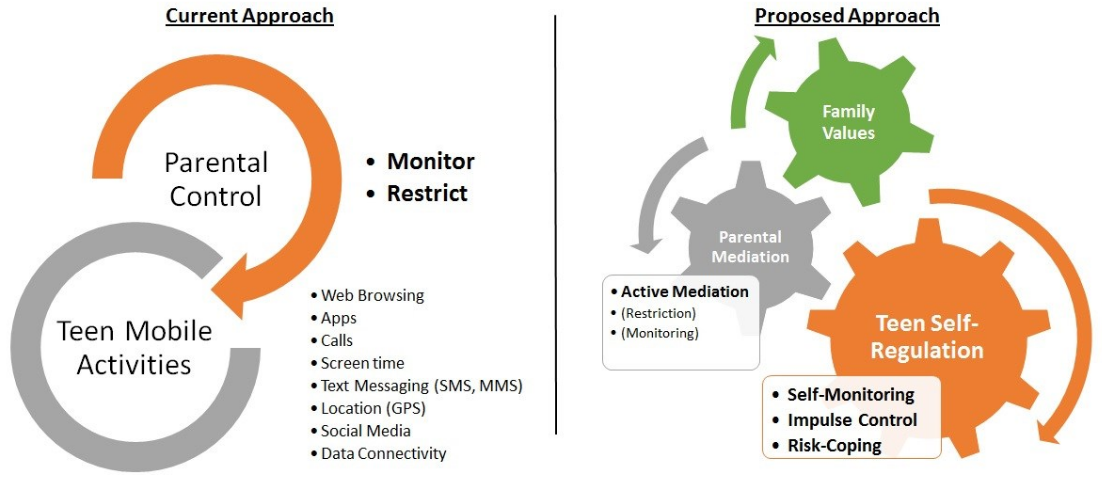
\includegraphics[width=1\textwidth]{Figures/current-vs-proposed}
\decoRule
\caption{Current versus Proposed Approach for Online Safety Apps}
\label{fig:current-vs-proposed}
\end{figure}

%----------------------------------------------------------------------------------------

% Chapter 2

\chapter{Content-control software and providers} % Main chapter title

\label{Chapter2} % For referencing the chapter elsewhere, use \ref{Chapter1}

Content control policies can be implemented at different levels. Some ISPs offer parental control options and even parental control software, other content control systems are integrated with the operating system, such as MacOS, which offers parental controls for some applications (Mail, Finder, iChat, Safari). The two major forms of content filtering technology are application gateway and packet inspection. The application gateway is called web-proxy for HTTP access and works by inspecting the request and the returned page using some rules and deciding if it should return the response. The packet inspection technique does not interfere with the connection, but inspect the data as it goes past and may decide at a later point to disconnect the client, by inject a TCP-Reset or similar faked packet. A combination of these two techniques is very popular because it allows more detailed filtering and can significantly reduce the cost of the system.

We will present next some parental control application and their features, on which we will try to build our system by taking a more self-regulatory approach.

\section{Net Nanny}

Net Nanny provides a content-control software as a way to monitor and control children's computer activity. The main features include blocking and filtering Internet content, place time limits on use and block PC games. Websites are blocked by content rather than URL, preventing children from accessing blocked websites through proxy websites. It is available on desktop platforms, Windows and Mac, and also on mobile platforms, Android and iOS, but the features and usability is not consistent on all platform, with some key features lacking on the mobile. It uses a dynamic filter that scans and analyses each web site to determine if it is appropriate for a child, based on a unique customization done by the parent. All the initial configuration is done online and it enforces the rules via a local client on each device it is installed. For each client, you can select from 4 profiles: Child, Pre-Teen, Teen and Adult, which can be further customized. \parencite{netNannyFeatures}

\subsection{Content Filtering}

Content filtering is the most used feature in all parental control systems and Net Nanny filters by analyzing the content for each web page in real time. Each site is matched against 17 objectionable categories, and each child profile have different level of blocking. Some categories are not completely blocked for some profiles, but the parents get a notification when the child visit sites in these categories. Parents can also create custom rules, to temporary allow access for some devices, and whitelists and blacklists for each child, to always allow or block certain websites. We follow the same approach by creating two classes of users for domain filtering and use a custom blocking mechanism to block certain domains for children, while allowing them for parent users.

\subsection{Internet Time Scheduling}

Children's internet use can be controlled in two ways using Net Nanny, by creating weekly schedules in half-hour increments, and you can also create weekly allowance duration in one-hour increments. This system does not depend on the system clock, so it cannot be bypassed. But it would be more useful to have more granularity when setting time limits, that's why we support 15-minute increments allowance periods for each day.

\subsection{Email notifications}

Net Nanny have two types of email notifications enabled. The first type of notification is sent when a child request a blocking exception for a specific domain, and the other one is in the form of a weekly summary. You can configure to get notification for multiple types of events, when a child hits a blocked site, continues after a warning or request a change in the blocking status. It would be more useful to have multiple options of getting notified about certain events occurring in the system, that's why we introduced mobile notifications into our system.

\subsection{Detailed Reporting}

Net Nanny offers an online console where you can view all the activity reports. You can view the activity by day, week and month, but not older than 30 days. It shows the blocked content in a pie chart, with some more information on mouse over. The report goes as deep as to show the page title, the time stamp and the user for each URL visited on a specific device. we do not include any type of reporting, because we thing that it would be a privacy issue for the child, since we try to implement a self-regulation system. All the discussion should be done in the family and the child should be warned about visiting certain domains, but not by checking every move he makes online. That's why we don't include any location related features, and Net Nanny does not support location either, but some other parental control systems do.

\subsection{Mobile Support}

The mobile support for Net Nanny is similar to the desktop experience, with some limitations. For the system to work, all the browsing should be done through the proprietary browser offered. On the iPhone the features are even more limited, because it does not interact with other apps and services at all. Since we started developing for mobile first and we try to keep the application features decoupled from the client device and system, we should not suffer of these limitations and we provide a seamless experience on both mobile platform, Android and iOS. \parencite{netNannyPCMag}

\section{Qustodio}

Qustodio is a parental control tool that runs on any device, from PC to Android and iOS and even on Kindle devices. It has a lot of features, from web content filtering, app blocking and detailed activity logs. The configuration and monitoring is handled either through an online dashboard or a mobile control application. For configuration, you need to install a local client on every device and assign a child's profile. The Windows desktop client has even an option to hide the Qustodio install, but we do not support this kind of approaches, and that's way we choose to not hide the parental control app in any way, because there's a fine line between spying and parenting and when trying to follow a self-regulatory approach, conversation and transparency are more important. The process of registering the mobile app involves assigning an existing or a new child profile and a name for the device, and specifying whether it is a parent or a child device. We use the same registration process for a device and we also have 2 types of users, a parent and a child, each class having access to different features.

\subsection{In-Depth Reports}

You can use the online dashboard to get up to date reports, or you can get an email with the daily activity summary for each child. The usage overview for search, web, social, app and device is shown in an interactive chart, with information specific to each category, such as interactions on Facebook and visited URLs. There is also support for creating rules, such as web browsing rules, application rules and time-usage limits.

\subsection{Web Filtering}

The default configuration blocks all access for websites from ten undesirable categories, among them Drugs, Gambling, Pornography and Violence, and other 19 categories are available for more fine tuning. You can also configure an automatic notification when blocking a site. The content filtering is not dependent on the browser used and uses real-time analysis to supplement category database. It can also block HTTPS content, so it cannot be bypassed using an anonymizing proxy, but it does not have a feature to request temporary access for some blocked sites.

\subsection{Time Usage Limits}

You can control the usage by defining a weekly schedule in one-hour increments per device or by setting a daily maximum for each day. The time tracking is done cross device, so you can make sure that a child does not exceed its daily limits. The system can also block the device, not just control its internet access. Access to any mobile application can be blocked, with some limitations on iOS. Time limits can be controlled at the application level, so you can limit the amount of time the child spends on certain social media apps during the school week.

\subsection{Social Monitoring and Location Reporting}

Social media monitoring on Qustodio is limited to Facebook. You can see the child's Facebook wall activity on the online dashboard, including posts, pictures and comments, as well as the identity of any friends involved in online chats, but it does not report the content of those chats, to maintain some degree of privacy. It also includes location-reporting features, which you can use to check the child's location as often as every five minutes.

\subsection{Mobile Support}

%---------------------------------------------------------------------------------------- 
% Chapter 3

\chapter{A self regulation approach} % Main chapter title

\label{Chapter3} % For referencing the chapter elsewhere, use \ref{Chapter1}

We started working on our system as a solution for parents who wanted a reliable parental control system, which tries to use the newest discoveries related to parental control impact on child development and is also easy to install and use. Most of the existing parental control systems are subscription based and work by creating a custom configuration for a specific family and enforcing the rules by using a client application for each target device. We wanted to design our system such that the user is in full control of the system configuration and all the data is kept locally, because we saw no point in getting the data outside the house, since its only use is only inside the local network, at least for out system. The system that we developed does not require any kind of client configuration, all the configuration needed is done on the central node, which in out case is a Raspberry Pi, which is an access point and a system control node, and a mobile application which the parents use to configure the parental control policies. We also offer a client application design for children devices, but that is only to extend the basic functionality and to also help with some initial configuration. So we basically moved the configuration part from the clients to the central node of the system. We tried to make the configuration as simple as possible, such that even a non-technical person can configure and start the system. The only commercial level alternative control parental system that we found using the same approach is Circle With Disney, whose details we presented in \ref{Chapter2}. It uses an additional network device which you have to purchase and it work by connecting to the local wireless network and using a technique called ARP Spoofing, used mostly for network attacks, because it aims to associate and attacker's MAC address with the IP address of another host, such as the default gateway, causing any traffic meant for that IP address to be sent to the attacker instead. Because we are building out system around the access point, instead of using an additional device, we have much more flexibility in the techniques we use for filtering and blocking at potentially a higher cost for the device. Any type of network device with a wireless card can be used to establish this kind of setup, but we used a Raspberry Pi because it is a cheap device, having almost the same price as a good router, and is quite powerful and flexible. Another difference between out approach and the Circle device is that the core of system is built around the  Domain Name System, by using a local DNS server for filtering and blocking. For this test we are using the open source project Pi-hole, which uses the DNS forwarder and DHCP server Dnsmasq to create the blocking and filtering system, which serves the primary scope of blocking all ads. Other tools that we used to develop out system are Flutter, an open-source mobile application development SDK created by Google, to make the mobile control application available on both Android and iOS and the Netfilter framework for more fine control on the network traffic on the access point. The tools and technologies used are as follows:

\begin{itemize}
\item Raspberry Pi 3 - as the access point and main controller
\item Pi-hole - for blocking and filtering
\item Dnsmasq - as DNS forwarder
\item Netfilter - to control the traffic on the access point
\item Go lang - the create a REST server for the mobile application
\item Flutter - to implement the cross-platform mobile application
\end{itemize}

We will next present the principles behind each of these components of the system and detail how they all work together to make the parental control task easy for the parents and beneficial for children development.

\section{Raspberry Pi}

Raspberry Pi is a series of small single-board computers developed in the United Kingdom by the Raspberry Pi Foundation to promote the teaching of basic computer science in schools and in developing countries. \parencite{raspberryPi} All models feature a Broadcom system on chip (SoC) with an integrated ARM compatible central processing unit (CPU) and on-chip graphics processing unit (GPU). The model that we used for our setup is a Raspberry Pi 3 Model B, released in February 2016 with a 64 bit quad core processor and on-board WiFi, Bluetooth and USB capabilities. The presence of on-board WiFi card makes it suitable to run as an access point, the computing power is enough to run the setup that we need, the DNS forwarder and other tools. It also offers a rich software package, with multiple Linux-based operating system to choose from, the recommended version being Raspbian, a Debian-based system, which we use in our setup. The software community around the Raspberry Pi boards is also very active, which helps a lot in development and in troubleshooting any problems along the way. The Pi-hole system that we integrated into our system was also developed into this community and created the opportunity for us to take it a step further and extend it by integrating the parental control features into it.

\section{Pi-hole}

Pi-hole is an Linux application which block advertisements and internet trackers at the network-level, by acting as a DNS sinkhole, and also DHCP server, on a private network. A DNS sinkhole is the name gives to a DNS server that gives out false information to prevent the use of a certain domain name. It was designed for use on embedded devices with network capabilities, such as the Raspberry Pi. It has the ability to block traditional adverts on websites, but also adverts in other places, such as smart TVs and mobile operating systems. It works by serving as a DNS server for a private network and using a list of advert and tracking domains from predefined sources that the system uses to compare DNS queries to. \parencite{salmela2015pihole} If a match is found in one of the block lists, Pi-hole will refuse to resolve the requested domain. This feature can be used to block any domains, not the advertisement ones, by extending the block list. We use this feature to block domains that are not considered useful for a child, such as social media platforms. You can also manually whitelist a domain, such that it is never blocked, and you can use the Pi-hole system to view reports about the DNS queries done by the clients.

\subsection{How it works}

Pi-hole acts as a forwarding DNS server, so if it does not know where a domain is it forwards the query to another server. When you configure it, it knows where the ad-serving domains are, because they are all in the local list, along with all the explicitly blocked domains, so it does not have to forward those requests. But it does not know where the legitimate domains are, so those requests are forwarded to an upstream, recursive server. Those servers also don't know where it is only if they were asked to find it before, the only DNS servers that truly know where a domain is are the authoritative DNS servers. The flow of events that are triggered when Pi-hole receives a DNS query can be seen in the figure below.\parencite{salmela2017ftldns}

\begin{figure}[th]
\centering
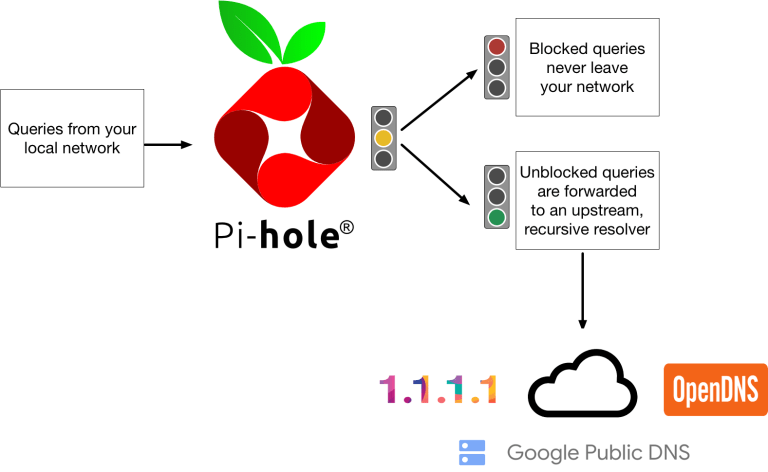
\includegraphics[width=1\textwidth]{Figures/pihole-dns}
\decoRule
\caption{The flow of traffic through the Pi-hole system}
\label{fig:circle}
\end{figure}

The flow of traffic goes like this:
\begin{enumerate}
\item The client asks the Pi-hole who is pi-hole.net
\item Pi-hole will check the cache and reply if the entry is present in the cache
\item Pi-hole will check the blocking list and if the domain is blocked, it will replay accordingly
\item If neither 2 or 3 are true, Pi-hole forwards the request to the external upstream DNS server, that was configured on installation
\item After receiving the answer from the upstream server, Pi-hole will reply to the client
\item Pi-hole save the answer in the cache to be able to respond more quickly if the same domain is queried again
\end{enumerate}

Pi-hole can also act as a network monitoring tool, since it logs all DNS queries sent to it, by default, so you can find what kind of traffic is going through your network. We integrated a component for visualizing this data into our system, to be able to quickly tell what domains are most visited by the children and what blocked domains they are trying to access. This integration was made easier by the fact that Pi-hole has a component which takes the raw data from the logs and pre-process it, storing it in a local database, to be able to serve quickly the types of queries needed, such as the top visited domains and the top blocked domains. We access this data by using a socket and some predefined commands. Pi-hole offers also a web interface to view these detailed reports. You can see the query types over time, forward destination over time, top domains, top blocked domains and other useful reports, as can be seen in the figure below.

\begin{figure}[th]
\centering
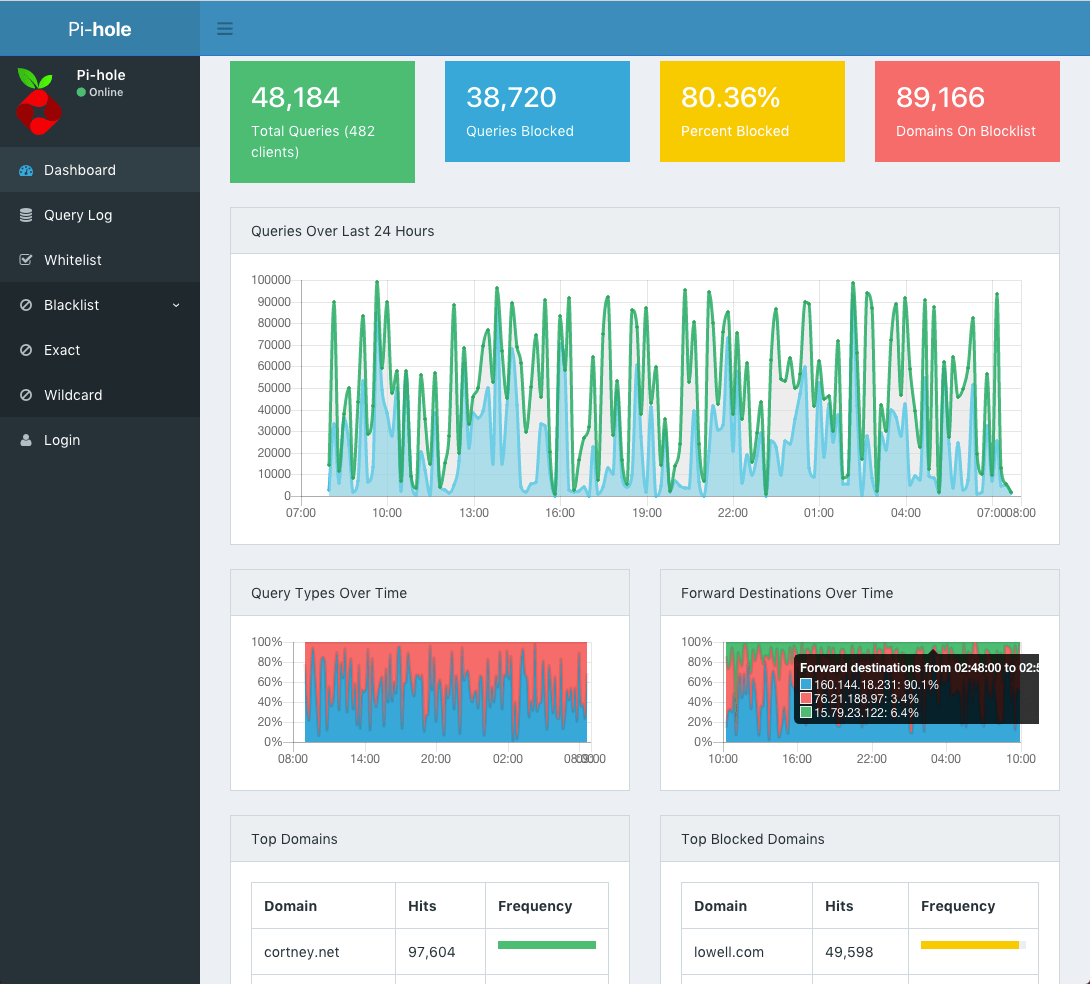
\includegraphics[width=1\textwidth]{Figures/pihole-admin}
\decoRule
\caption{The Pi-hole admin dashboard}
\label{fig:circle}
\end{figure}

Other benefits that Pi-hole brings to your local network are related to bandwidth and network speed. Because it works at the DNS level and prevents the ads and blocked domains from being downloaded. Since these ad images, videos and sounds are not being downloaded, the network will perform better. For the same reasons, it also reduces bandwidth, by preventing undesired assets from being downloaded. You can also extend the default block list to include sites that are known to serve malware or act as a phishing site, which brings another level of security, very important in the context of children using the Internet. The performance should not be a problem for the Pi-hole system, since even a not so powerful Raspberry Pi has been documented of handling up to 60 clients without problems, more than enough for a family network. \parencite{salmela20177things}

\section{Dnsmasq}

Dnsmasq is a lightweight and easy to configure DNS forwarder and DHCP server. It can be used to serve names for local machines which are not in the global DNS and is designed to offer DNS and DHCP solutions for small networks. \parencite{debianHowToDnsmasq}
It has low resource requirements for system resources, so it is a good solution for our Raspberry Pi setup. It improves the performance and reduces the load on upstream DNS servers by caching DNS records locally.

Dnsmasq loads the content of /etc/hosts file to be able to resolve local names, and that allows some useful tricks, such as overriding some global domains, by adding a line with the format "0.0.0.0 annoyingsite.com". This prevents the domain annoyingsite.com from being resolved and that's the way Pi-hole uses it to block ads, by creating an entry for each known ad serving domain, and we also use that to block any other unwanted domains. Pi-hole keeps this Dnsmasq related configuration in a file named gravity.list, which is updated periodically to include the newest ad domains. It currently contains around 126000 of ad domains and the number is constantly growing. We can see below some of the line from this files, with 10 blocked ad serving domains.

\begin{lstlisting}
192.168.0.103 zxypenguin.people-group.su
192.168.0.103 zy.zeroredirect1.com
192.168.0.103 zyban-store.shengen.ru
192.168.0.103 zyban.1.p2l.info
192.168.0.103 zyban.about-tabs.com
192.168.0.103 zybezradio.com
192.168.0.103 zyiztazhfprochain.review
192.168.0.103 zyjyyy.com
192.168.0.103 zyngatables.com
192.168.0.103 zyngawithfriends.com
\end{lstlisting}

The included DHCP server functionality supports static and dynamic DHCP leases, multiple networks and IP address ranges. We define a DHCP range for our network, along with the upstream DNS servers to use. The defined upstream DNS servers are the Google one and the configuration for this looks as follows:

\begin{lstlisting}
server=8.8.8.8
server=8.8.4.4
interface=wlan0
dhcp-range=10.0.0.2,10.0.0.5,255.255.255.0,12h
\end{lstlisting}

Other Dnsmasq feature that is for use for us is that it can support different DNS server configuration for different DHCP settings. We are using this to establish the way the two classes of users defined in out system can access the network, since we don't want to apply the same blocking rules for the parents as for the children. Dnsmasq supports defining a different DNS resolver based on MAC address, and we use that to allow the parent's device to bypass the domain blocking rules that apply only to children devices, by configuring the system to use the Google resolver for that devices. That is easily done by adding the following rules to the Dnsmasq configuration:

\begin{lstlisting}
## This will go straight to Googles DNS Servers.
dhcp-option=tag:googlesdns1,6,8.8.8.8
dhcp-option=tag:googlesdns2,6,8.8.4.4

## This will go straight to Opendns Servers.
dhcp-option=tag:opendns1,6,208.67.222.220
dhcp-option=tag:opendns2,6,208.67.222.222

## Your Device that goes to Google DNS
#dhcp-host=dc:0b:34:cc:b0:ff,set:googlesdns1 #Nexus

## Your Device that goes to OpenDNS
#dhcp-host=a8:b8:6e:41:0e:de,set:opendns1
#dhcp-host=f8:23:b2:ad:4d:f3,set:opendns1
\end{lstlisting}

We can configure that to work with different devices and DNS servers, to add another level of control over the blocking features. \cite{archwikiDnsmasq}

\section{Netfilter}

\section{Go Lang}

\section{Flutter}

\section{All together}

%----------------------------------------------------------------------------------------

%----------------------------------------------------------------------------------------
%	THESIS CONTENT - APPENDICES
%----------------------------------------------------------------------------------------

\appendix % Cue to tell LaTeX that the following "chapters" are Appendices

% Include the appendices of the thesis as separate files from the Appendices folder
% Uncomment the lines as you write the Appendices

%% Appendix A

\chapter{Frequently Asked Questions} % Main appendix title

\label{AppendixA} % For referencing this appendix elsewhere, use \ref{AppendixA}

\section{How do I change the colors of links?}

The color of links can be changed to your liking using:

{\small\verb!\hypersetup{urlcolor=red}!}, or

{\small\verb!\hypersetup{citecolor=green}!}, or

{\small\verb!\hypersetup{allcolor=blue}!}.

\noindent If you want to completely hide the links, you can use:

{\small\verb!\hypersetup{allcolors=.}!}, or even better: 

{\small\verb!\hypersetup{hidelinks}!}.

\noindent If you want to have obvious links in the PDF but not the printed text, use:

{\small\verb!\hypersetup{colorlinks=false}!}.

%\include{Appendices/AppendixB}
%\include{Appendices/AppendixC}

%----------------------------------------------------------------------------------------
%	BIBLIOGRAPHY
%----------------------------------------------------------------------------------------

\printbibliography[heading=bibintoc]

%----------------------------------------------------------------------------------------

\end{document}  
